\section{Motivational Example}
\label{sec:motivation}

To show that designing an optimal memory system for energy efficiency of the entire ASIP, we analyze a kernel in a streaming application. We chose \textit{discrete cosine transform (DCT)} kernel of the streaming application \textit{MP3} encoder. The experimental setup will be described in detail in Section \ref{}. Figure \ref{fig:cis-mem} shows the core and total energy consumption of the various customized versions of \textit{DCT} for a fixed cache size. {\bf to do: define core energy and memory}. The customized versions are sorted according to the decreasing order of the execution time (i.e) the execution time of $custom_i$ < $custom_j$, if \begin{math}i<j\end{math}. It is evident from the Figure \ref{} that the total energy consumption of the system does not follow the same trend as the core energy consumption. For example, $custom_3$ has lower core energy compared to $custom_2$ but the total energy follows the other trend. Thus, an holistic approach is required in selecting appropriate custom instructions and memory subsytem in designing energy efficient ASIP system. 
\begin{figure}[h]
\center
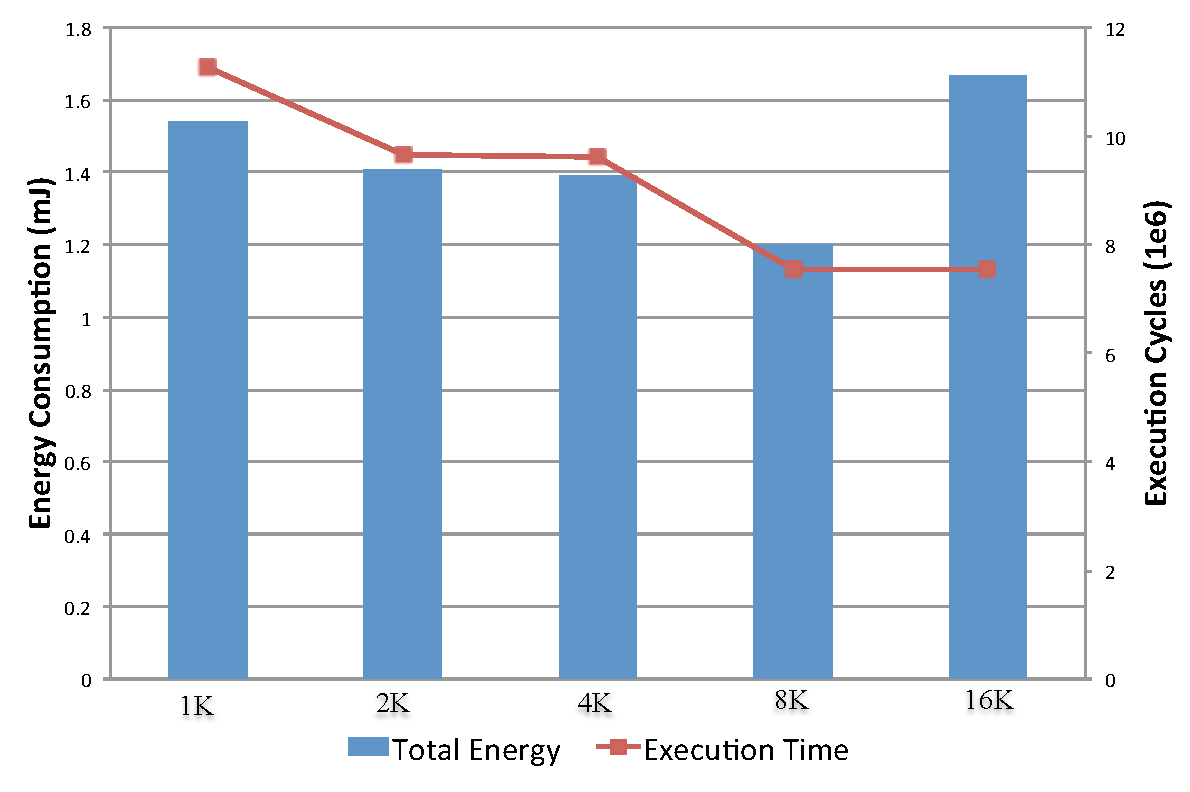
\includegraphics[width=0.36\textwidth]{cache-size.pdf}
\label{fig:cache-size}
\caption {Impact of various cache size on a particular customized version}
\end{figure}

Figure \ref{fig:cache-size} illustrates the effect of the various cache sizes of a particular customized version of \textit{DCT} on the total energy consumption and execution time. We modify the instruction cache sizes from 1KB to 16KB. In terms of performance, the most optimal cache size is 16KB. With insignificant performance loss, the optimal cache in terms of energy is 8KB. Furthermore, area saving by going from 16KB to 8KB is significant (from Table \ref{} ). It is very important for the designer to choose the appropriate cache size for the most efficient energy ASIP system. 

In our framework along with custom instruction and cache size selection, we also incorporte voltage/frequency scaling to improve the energy. Just by considering any of the techniques individially may result in a local optima. Thus, it is important to consider all the three techniques collectively to reach a global optimal point. To justify this claim, we have provided extensive results in Section \ref{sec:experiment}.  
